% Compile with: uplatex file.tex && dvipdfmx file.dvi
%           or: latexmk -uplatex file.tex
\documentclass[dvipdfmx]{article}
\usepackage{amsmath, amssymb}
\usepackage{tikz}

\title{scenario\_lattice\_figures}
\date{\today}

\begin{document}
\maketitle

On a $3\times3$ honeycomb lattice (open boundaries), expand the sum $\sum_{\langle ij\rangle}S_i^zS_j^z$ over nearest-neighbor site pairs $\langle ij\rangle$ into the actual bonds (adjacent pairs).

Expand the nearest-neighbor sum of $Sz_i$ $Sz_j$ over a 3x3 honeycomb lattice

\begin{equation}
  Sz\left(8\right) Sz\left(9\right)+Sz\left(7\right) Sz\left(8\right)+Sz\left(5\right) Sz\left(8\right)+Sz\left(5\right) Sz\left(6\right)+Sz\left(3\right) Sz\left(6\right)+Sz\left(4\right) Sz\left(5\right)+Sz\left(1\right) Sz\left(4\right)+Sz\left(2\right) Sz\left(3\right)+Sz\left(1\right) Sz\left(2\right)
  \label{eq:E1}
\end{equation}

\begin{center}
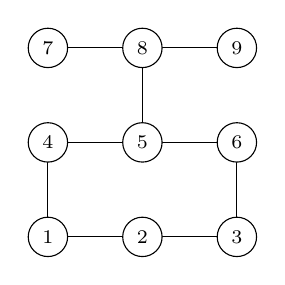
\begin{tikzpicture}[scale=1.2, site/.style={circle,draw,fill=white,inner sep=1pt,minimum size=5mm,font=\scriptsize}]
  \draw (0.000,0.000) -- (1.000,0.000);
  \draw (1.000,0.000) -- (2.000,0.000);
  \draw (0.000,1.000) -- (1.000,1.000);
  \draw (1.000,1.000) -- (2.000,1.000);
  \draw (0.000,2.000) -- (1.000,2.000);
  \draw (1.000,2.000) -- (2.000,2.000);
  \draw (0.000,0.000) -- (0.000,1.000);
  \draw (1.000,1.000) -- (1.000,2.000);
  \draw (2.000,0.000) -- (2.000,1.000);
  \node[site] at (0.000,0.000) {1};
  \node[site] at (1.000,0.000) {2};
  \node[site] at (2.000,0.000) {3};
  \node[site] at (0.000,1.000) {4};
  \node[site] at (1.000,1.000) {5};
  \node[site] at (2.000,1.000) {6};
  \node[site] at (0.000,2.000) {7};
  \node[site] at (1.000,2.000) {8};
  \node[site] at (2.000,2.000) {9};
\end{tikzpicture}
\end{center}

Save the bond structure of the lattice sum just computed as a figure (SVG and standalone TeX, plus PDF if available). The figure lets you confirm that the intended lattice and boundary conditions were used.

Save the lattice figure

Now expand the same nearest-neighbor sum on a $3\times3$ square lattice, this time under periodic boundary conditions. The bonds that wrap around due to the periodic boundary are drawn as dashed lines in the figure to distinguish them.

Expand the nearest-neighbor sum of $Sz_i$ $Sz_j$ over a 3x3 square lattice with periodic boundary conditions

\begin{equation}
  Sz\left(8\right) Sz\left(9\right)+Sz\left(7\right) Sz\left(9\right)+Sz\left(6\right) Sz\left(9\right)+Sz\left(3\right) Sz\left(9\right)+Sz\left(7\right) Sz\left(8\right)+Sz\left(5\right) Sz\left(8\right)+Sz\left(2\right) Sz\left(8\right)+Sz\left(4\right) Sz\left(7\right)+Sz\left(1\right) Sz\left(7\right)+Sz\left(5\right) Sz\left(6\right)+Sz\left(4\right) Sz\left(6\right)+Sz\left(3\right) Sz\left(6\right)+Sz\left(4\right) Sz\left(5\right)+Sz\left(2\right) Sz\left(5\right)+Sz\left(1\right) Sz\left(4\right)+Sz\left(2\right) Sz\left(3\right)+Sz\left(1\right) Sz\left(3\right)+Sz\left(1\right) Sz\left(2\right)
  \label{eq:E2}
\end{equation}

\begin{center}
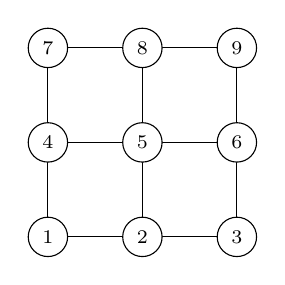
\begin{tikzpicture}[scale=1.2, site/.style={circle,draw,fill=white,inner sep=1pt,minimum size=5mm,font=\scriptsize}]
  \draw (0.000,0.000) -- (1.000,0.000);
  \draw (1.000,0.000) -- (2.000,0.000);
  \draw[dashed] (2.000,0.000) -- (0.000,0.000);
  \draw (0.000,1.000) -- (1.000,1.000);
  \draw (1.000,1.000) -- (2.000,1.000);
  \draw[dashed] (2.000,1.000) -- (0.000,1.000);
  \draw (0.000,2.000) -- (1.000,2.000);
  \draw (1.000,2.000) -- (2.000,2.000);
  \draw[dashed] (2.000,2.000) -- (0.000,2.000);
  \draw (0.000,0.000) -- (0.000,1.000);
  \draw (0.000,1.000) -- (0.000,2.000);
  \draw[dashed] (0.000,2.000) -- (0.000,0.000);
  \draw (1.000,0.000) -- (1.000,1.000);
  \draw (1.000,1.000) -- (1.000,2.000);
  \draw[dashed] (1.000,2.000) -- (1.000,0.000);
  \draw (2.000,0.000) -- (2.000,1.000);
  \draw (2.000,1.000) -- (2.000,2.000);
  \draw[dashed] (2.000,2.000) -- (2.000,0.000);
  \node[site] at (0.000,0.000) {1};
  \node[site] at (1.000,0.000) {2};
  \node[site] at (2.000,0.000) {3};
  \node[site] at (0.000,1.000) {4};
  \node[site] at (1.000,1.000) {5};
  \node[site] at (2.000,1.000) {6};
  \node[site] at (0.000,2.000) {7};
  \node[site] at (1.000,2.000) {8};
  \node[site] at (2.000,2.000) {9};
\end{tikzpicture}
\end{center}

\end{document}